%!TEX TS-program = XeLaTeX
\documentclass[twoside]{article}
\usepackage{fontspec,lipsum}
\defaultfontfeatures{Ligatures=TeX}
\usepackage[small,sf,bf]{titlesec}
\usepackage[a5paper]{geometry}
\usepackage{hyperref}
\usepackage{graphicx}
\usepackage{xltxtra}
\setlength{\parindent}{0cm} 
\setlength{\parskip}{2mm}
\defaultfontfeatures{Scale=MatchLowercase}
\setmainfont[Numbers=OldStyle]{Minion Pro}
\setmonofont{Monaco}
\setsansfont{Myriad Pro}
 
\begin{document}

\newgeometry{left=0cm,bottom=1.5cm,right=0cm}
\thispagestyle{empty}
\begin{center}
\Huge


\includegraphics[scale=0.6]{exetercrestsmall.png}

Fresher's Guide

\textsc{exeter mcr}

{\large \it
Staircase 8, Exeter College, Turl Street, Oxford, England}
\vfill
\large

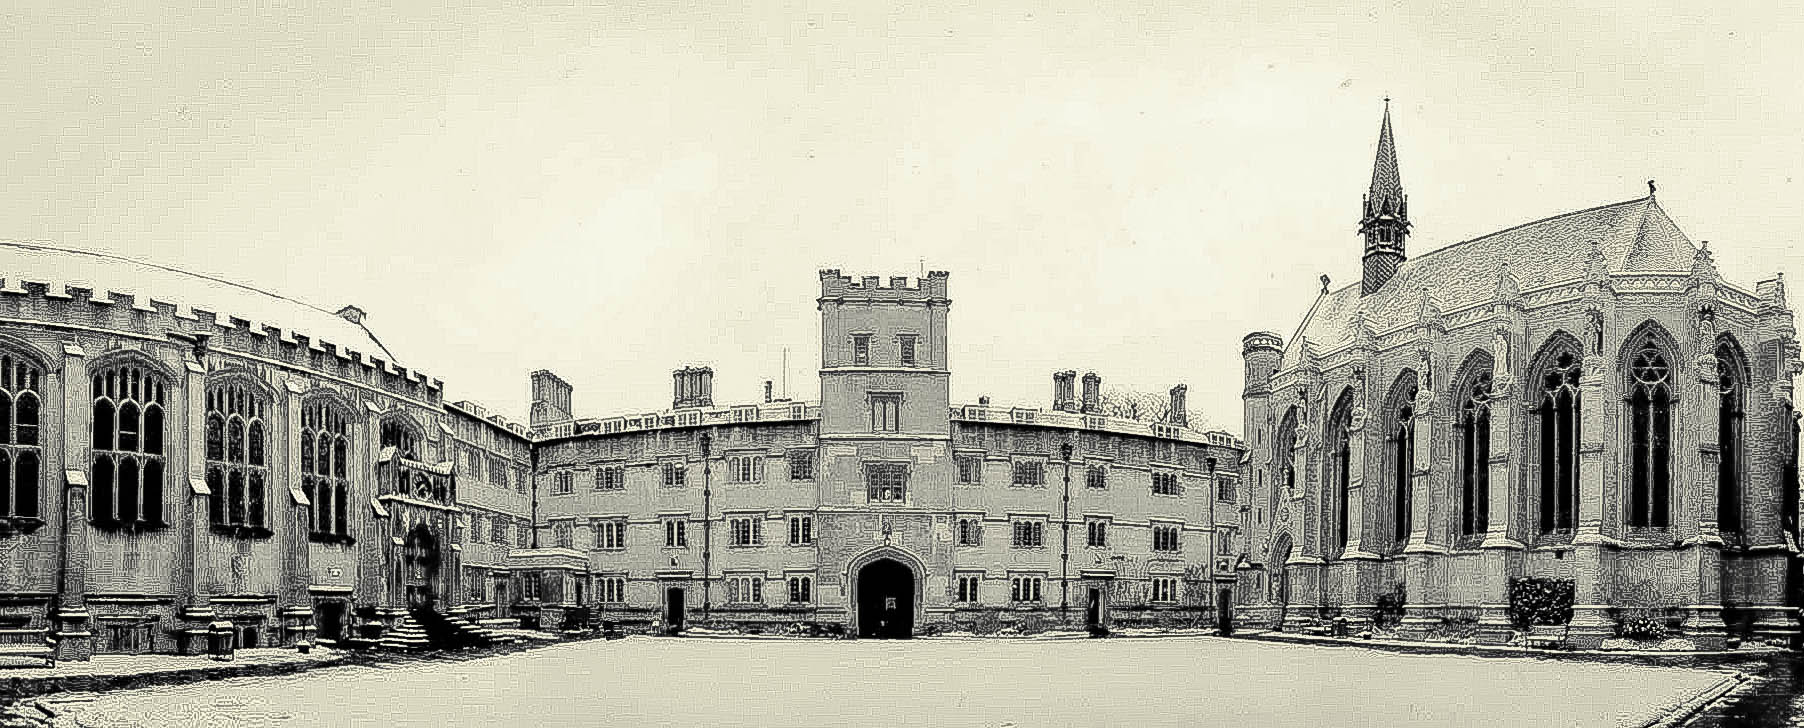
\includegraphics{background.jpg}

\textsc{october 2013}
\end{center}

\restoregeometry
\pagebreak
\newpage
\thispagestyle{empty}
\mbox{}
\pagebreak

There are many guides available for new students in Oxford. Different
versions are provided by OUSU (the Oxford University Student Union), the
faculties, the colleges, the common rooms, and other organisations. As
there is plenty of information out there, we did not try to make a
comprehensive document. However, we designed this guide to focus on two
things: first, on what we think are the most important and urgent things
for new students to know and do and, second, on the little details that
we wish we knew as new students, and which in our opinion can make all
the difference.

{\sffamily
\tableofcontents
}

\section{Before you arrive}\label{before-you-arrive}

\subsection{Vaccinations}\label{vaccinations}

Two important vaccines for people coming to the UK are MMR (Measles,
Mumps, Rubella) and Meningitis C. In line with national policy, the
University recommends that two MMR vaccinations (this does not include
the MR vaccine) are received before arrival; they can be received a
month apart. Similarly, national policy is that any unvaccinated
individual attending university, irrespective of age, should be
immunised with the Men C vaccine before they enrol or as soon as
possible thereafter.

Further information about vaccinations is on the Exeter College Graduate
Freshers' Weblearn site, and on these pages on Mumps
(\url{http://www.ox.ac.uk/students/shw/health/mumps/}) and Men C
(\url{http://www.ox.ac.uk/students/shw/health/meningitis/})

\subsection{Border crossing}\label{border-crossing}

Carry all the immigration documents that you used to apply for the UK
visa with you in your hand luggage. There have been stories about
international students being asked to produce all of these on their
first entry into the UK. For more information about immigration, see the
UK Border Agency site \url{http://www.ukba.homeoffice.gov.uk}.

\subsection{Money}\label{money}

It might take a little bit of time to open a bank account, so make sure
you have access to enough GBP to get through the first little while.
Most cash points in Oxford won't charge you a fee for making an ATM
withdrawal with a non-UK card, although your home bank will probably
impose a transaction fee.

If possible, open a UK bank account before you come. (There is more
information below on how to open a bank account.)

\subsection{Transport to Oxford}\label{transport-to-oxford}

Oxford is very well-connected to London and the airports by bus and
train.

\paragraph{From London}\label{from-london}

If you are coming from London City, the fastest way is to take a train
from Paddington. These run frequently during the day (every half hour or
so), and take about an hour. For schedules, see
\url{http://www.nationalrail.co.uk}. The cost will differ depending on
the tariff, and what rail cards you have. Peak time is very expensive
(early mornings and late afternoons), but a standard off-peak ticket
will cost a little over �20. To get from the railway station to Exeter
House, either take a Number 3 bus (the stop closest to Exeter House is
outside the Magdalen Arms pub), or a taxi (a taxi will cost about �10,
and taxis are always available at the railway station). From 30
September, the Number 3 bus is being extended to start at the Oxford
Railway Station, so there will be a direct bus from Exeter House to the
Railway Station from then onwards.

It's also possible to take the bus from London to Oxford. There are two
services, going from Victoria Station and picking up in central and West
London: the \href{http://www.oxfordtube.com}{Oxford Tube} and the X90.
These services are cheaper than the train; an adult one-way ticket is
�13 (return �16). Although the bus takes longer (at least an hour and a
half), it stops closer to College and Exeter House than the train does.
For College, you could get off either at the High Street or at the
terminus (Gloucester Green). For Iffley the stop you need is
St.~Clement's, which is a short taxi ride or 15-minute walk from Exeter
House. Alternatively, you could get off at the High Street, cross the
road, and take \textbf{Bus \#3} (which leaves from opposite the Queen's
College) to the Magdalen Arms, which is next to Exeter House.

These buses and trains are also relevant should you want to go to
London! If you plan to travel regularly by train it is worth investing
in a young persons railcard (for 16 to 25 year olds). It costs �30 and
gives you a 1/3 off rail fare for a year. Similarly if you intend to use
the Oxford Tube service regularly you can purchase an Oxford Tube 12
pass which gives you 12 journeys for �60 making the journeys a little
bit cheaper.

The map on the next page shows the relevant bus stops as blue circles, with College
and Exeter House marked in yellow.

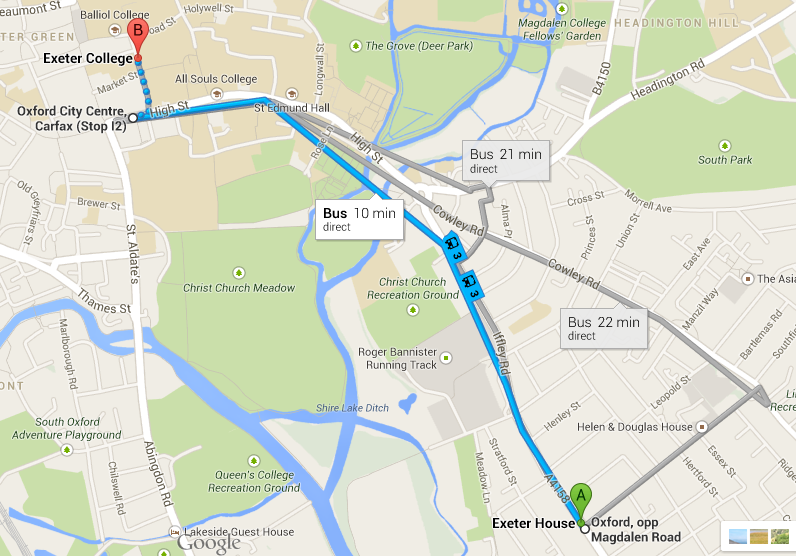
\includegraphics[scale=0.4]{exeter-house-dir.png}

\paragraph{From the airports}\label{from-the-airports}

The best way to get from the airports to Oxford is by bus. The Oxford
Bus Company runs the \textbf{Airline bus service} from both Heathrow and
Gatwick. The buses from Heathrow run every half hour during the day, and
from Gatwick they run every hour. The bus stops for arriving in Oxford
on the Airline are similar to those for the Oxford Tube or the X90.

If you are flying into either Luton or Stansted, the bus ride to Oxford
is longer (especially for Stansted), and is operated by National Express
(\url{http://www.nationalexpress.com}). It is also possible to transit
from these airports to London by train, though you'll have to change
between stations in London.

Another alternative is to fly to Birmingham or Southampton, both of
which cities are well-connected to Oxford by train.

\paragraph{Coming by car}\label{coming-by-car}

This can be tricky for central Oxford: Oxford's mediaeval street pattern
was not designed for motor cars. Many of the streets are one way, and
some streets that look open on the map are actually closed (enforced
either by physical barriers or by CCTV cameras and fines). The only way
to get to Exeter College's main site in Turl Street is via Parks Road
and Broad Street.

In coming to Oxford from the north, come down Banbury Road, and turn
left into Parks Road (if you get as far as St Giles' -- a very wide
tree-lined avenue -- you have gone too far and need to turn around).
Once on Parks Road continue to the traffic lights at the end of the
street (at the cross-roads next to the King's Arms), turn right into
Broad Street, then turn left into Turl Street: here is a map of the
route: \url{http://goo.gl/maps/9wwVx}.

From the East: St.~Clement's to High Street, right into Longwall Street
(with most of the traffic), the road turns left to become South Parks
Road, turn left at the junction into Parks Road, then right into Broad
Street at the King's Arms, and left into Turl Street:

Coming by car is much easier for Exeter House
(\url{http://exetermcr.org/exeter-house}, 235 Iffley Road): there are
barely any road restrictions, and even the road works are finally over!
However, parking at Exeter House is extremely limited, and the city's
parking wardens are very strict. Exeter House, in effect, provides no
parking for residents, which makes owning a car in Oxford very difficult
(cycling, however, is a very convenient way to get around -- see later
sections on this).

\section{What you can expect to find in the room, and what you might
want to
bring}\label{what-you-can-expect-to-find-in-the-room-and-what-you-might-want-to-bring}

For College accommodation, College provides all the usual essential
furniture. Notably, there will also be a pillow and a duvet in your room
and the wardrobe will have coat hangers included, so don't bring your
own if you don't mind using these. The shared kitchen is stocked with
plates, pots, pans, cutlery, a kettle, a toaster, a microwave, an oven
and a fridge and suffices for day-to-day cooking. Other than that, it's
largely up to you to decorate where you live and although it is College
policy that you can't stick stuff to the walls, a little creativity goes
a long way. Some of the things to further think about might be:

\begin{itemize}
\itemsep1pt\parskip0pt\parsep0pt
\item
  towels, bedding (sheets for a 90x200 cm mattress, pillow cases, a
  duvet cover)
\item
  electrical extension leads, converters to UK plugs (3-pin, 230V),
  clock, alarm clock, bedside lamp, headphones
\item
  specialist cooking utensils (blender, rice cooker, chop sticks, etc.),
  a kettle if you want to make tea in your room and do not want to go to
  the kitchen every time
\end{itemize}

For some a big relief: both your room and the kitchens will be cleaned
by College housekeeping staff, who are referred to as `scouts'. By
default, your room will be cleaned once a week (at most) and your bins
will be emptied every day. If you find this too intrusive or don't think
it is necessary every week or day, you could place your bin outside of
your door or just discuss with your scout some other mutually agreed
arrangement. They are very nice and a great help. They also vacuum and
clean the kitchens every morning on weekdays, which over time you will
come to appreciate tremendously. However, please be aware that it is not
the scout's job to make your bed, tidy your room or do the dishes, so
they won't do it. In general, moral hazard -- the phenomenon that you
lower your effort because somebody else cleans up the mess anyway -- is
a big trap, please try to avoid it if you can.

Overall, living in Exeter House is very comfortable. As it is modern, it
may lack some charm or the weight of an old architecture, but at the
same time you won't have to live in old squeaky, dusty and moist rooms,
as is the student stereotype. The bathroom is great (but check out the
light above the mirror as it is less unforgiving than the main light in
early mornings) and the heating works like a charm, things that
genuinely matter on another rainy day.

Formal dress deserves some special attention, as there are many
occasions in Oxford where you might be required to wear a suit or even
black tie: formal dinners, certain parties, special events, balls etc.
In fact, there are a surprising number of these occasions, and while
they are not compulsory, they tend to be very good fun.

A special kind of attire that you are guaranteed to need is `subfusc'.
This is the clothing ensemble worn for matriculation (the
university-wide ceremony of acceptance to the university), for sitting
exams (including viva voce exams for DPhil students), and for graduation
and as such it is the most official attire. Girls' sub-fusc has
traditionally consisted of a dark skirt or trousers, black stockings or
tights, black shoes, white shirt with collar and black ribbon tie. Boys'
has traditionally been a dark suit, white shirt, white bow-tie, dark
socks and black shoes. However, as of 2012, there is no actual
stipulation to wear gender-specific items should you wish not to. In
practice, this means that you can choose for yourself whether to wear a
skirt or trousers or suit, and you can choose for yourself whether to
wear the black string tie or the white bow tie, or a black necktie (but
your options are still constrained to wearing the items specified within
subfusc -- there is no chance to wear bright, colourful clothing!).
There will no longer be any distinction in subfusc between the sexes, so
just choose the clothing that you feel most comfortable with from the
options available.

Besides subfusc you will also definitely need `academic dress',
consisting of a `cap' and a `gown'. The `cap' could traditionally be a
`soft cap' for women, but these days virtually everyone has the
square-shaped `mortarboard': you have to wear your gown, and carry your
mortarboard, at University examinations and ceremonies (matriculation,
graduation).

The gown is used surprisingly often, for instance at special dinners.
The basic gown, if you are studying for a postgraduate degree at Oxford,
is called the Advanced Student's Gown (sometimes called the Graduate
Student's Gown). If you are studying for a second undergraduate degree
or for a diploma (even though you might be a graduate of another
University), then you wear the Commoner's Gown. This is the default
position; but there are a few variations, if you want to enjoy them:

\begin{itemize}
\itemsep1pt\parskip0pt\parsep0pt
\item
  If you have graduated from Oxford, then you are entitled to wear the
  Oxford gown (with, at University examinations and ceremonies, the
  hood) of your previous Oxford degree (or if you were an undergraduate
  scholar at Exeter you may continue to wear your undergraduate
  scholar's gown). So, if you have just graduated with a BA from Oxford
  (from any College), you can wear your BA gown instead of the advanced
  student's gown, and the BA gown and hood at your next graduation. If
  you are (or become) a DPhil student at Oxford who has already
  graduated with an Oxford Masters (MSt, MSc, MPhil, BCL, MJur, and so
  on), you are entitled to wear your Oxford Masters gown (and hood) in
  place of your advanced student's gown.
\item
  If you have not graduated from Oxford, but have a degree from any
  other University (except Cambridge University or Trinity College
  Dublin), then you are entitled to wear the gown (with, at University
  examinations and ceremonies, the hood) in which you graduated at your
  previous University.
\item
  If you have graduated from Cambridge University or Trinity College
  Dublin, then you can do something called ``incorporate'' your degrees.
  If you do this, you are entitled to wear at Oxford the same gown that
  you would have gained had you done your Cambridge/TCD degrees here at
  Oxford.
\end{itemize}

Do note that subfusc and academic dress officially are two separate
things (although they are often lumped together). To clear up some
further confusion: for many events (for example, the College's Graduate
Freshers' Dinner in Week 1 of Michaelmas Term) you need regular (formal)
clothing together with \emph{just your gown}, not with full subfusc as
described above and not with a mortarboard.

All of these items can be bought in Oxford, of course, and you will have
at least two weeks to do this -- this is the time from your arrival
until matriculation. Indeed, it's probably going to be easier to
purchase the gown, ribbon or bow tie, and mortarboard here, but it might
be cheaper to bring your own shoes, suit, skirt, shirts, etc. The gown
can be bought from a number of shops or on rare occasion borrowed from
College. The shop closest to Exeter College is Walters of Oxford,
located on Turl Street opposite Lincoln College; Shepherd \& Woodward
and Ede \& Ravenscroft are a couple of minutes' walk away on the High
Street. Expect to spend around �40 for the gown, mortarboard and tie,
and make sure you pick up the appropriate gown (the advanced student's
gown is knee-length, while the commoner's gown is hip-length).

Archaic as they may seem, the rules of subfusc are actively enforced, as
this gentleman's bold light sock adventure during exams clearly shows:

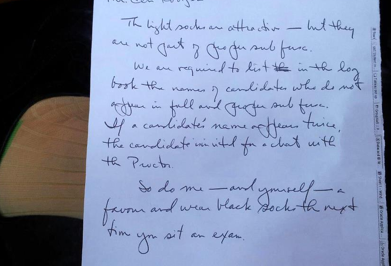
\includegraphics[scale=0.745]{light-sock-adventure.png}


\section{Semi-urgent admin upon
arrival}\label{semi-urgent-admin-upon-arrival}

There are a few things that need to be done over your first few days in
Oxford.

\subsection{Getting your Bod card}\label{getting-your-bod-card}

Your Bod card (officially called the ``University Card''), which is your
official university ID card, will be handed out by the college staff on
Wednesday of Freshers' Week at that day's induction session. However, if
you need it before that (and you probably will), you can come to College
Office to collect it. The College Office is in the far back corner of
College (ask at the College Porters' Lodge for directions).

The Bod card allows you access into the University and College buildings
-- including Exeter House -- and the MCR; you pay for food and drinks in
college with it; you take out library books with it; and it will be
checked when you sit exams. It is very important! If you ever lose your
card, then you need to request a new card: that is done via the College
Office (not via your Department and not direct to the University Card
Office), and there is a form on the College web-site to help you to
request a new card. If your card is stolen, then it is very important
that you report it stolen and request a replacement quickly, so that
whoever stole it is prevented from entering buildings and pretending to
be you. If you lose your card, then there is a fee to pay
(\url{http://www.admin.ox.ac.uk/card/lost/}) via the University store
for a replacement, which you have to pay in addition to requesting a new
card via College; if your card is stolen or damaged, then there is no
charge for a replacement.

\subsection{Activating your email address and connecting to the
internet}\label{activating-your-email-address-and-connecting-to-the-internet}

The College and the university should provide you with detailed guidance
and the required credentials to get you online. The process can be a bit
of a hassle, but it is very important to complete quickly, as email is
the main means of official communication. Please get in touch with the
College IT department (by e-mail at
\url{mailto:it-help@exeter.ox.ac.uk}, or at their office in the Balsdon
Room) or any of the MCR committee if you are unable to do this.

You will get two accounts: (1) an Oxford University username, for
anything related to the University and for a remote access account (for
accessing the University's wireless network, and for accessing
restricted resources if you live out of College or University
accommodation) and (2) an Exeter College login, purely for accessing the
College computers and for printing in College. Your Oxford University
username will be e-mailed to you by the University (not by Exeter
College) when your University contract has been returned and processed.

More information at
\url{http://www.exeter.ox.ac.uk/currentstudents/computing/internet/}.

\subsection{Register with the Police}\label{register-with-the-police}

International students from some countries need to do this immediately
upon arrival (it will say so on your visa if you need to register with
the police). The main police station is on St.~Aldates, about a
10-minute walk from the main College site. You'll pay �34 and get a
registration certificate, which you should keep safe. If you need to
register with the police on arrival, you'll also have to report any
official changes to the police to be recorded on your certificate, for
instance if you get a new passport, or if you change address during your
time in the UK.

The police have a registration desk at the University's International
Student Orientation Programme which saves you a trip to the police
station. More information at
\url{http://www.ox.ac.uk/students/international_students/visaduring/police/}.

Upon arrival, international students will also need to present passports
and visas to the College Office so they can scan them for their records.

\subsection{Open a bank account}\label{open-a-bank-account}

Life is very hard without a bank account (and something in it!). If you
have not worked or studied in the UK before (or have somehow managed
until now to do so without a UK current account), then you will need one
whilst at Oxford. To open one, you have two main options: (1) do it
whenever you like by going to the bank itself or (2) go to the
International Students' Orientation Programme (at Exam Schools,
\url{http://www.ox.ac.uk/students/new/orientation/}) or the Freshers'
Fair (this takes place in Freshers' Week), where representatives of the
whole range of banks will be present (more on the Freshers' Fair below).
In our experience, the banks' offers at the Fair are not different from
what they otherwise are.

To open a bank account, the main document you'll need is proof of
enrolment. The Freshers' pack you receive from college will have a
letter which you can take to the bank as proof of this. If the bank does
not accept this letter, you can print a more official one from the
Student Self-Services (\url{http://www.ox.ac.uk/students/}) though bear
in mind that to be valid it needs to be stamped with the college stamp,
which can be done at the College Office). If the bank asks for any other
documents, please email \url{mailto:college.office@exeter.ox.ac.uk} with
details of what the bank requires, to see if the College can help.

The banks are located mainly on Cornmarket Street (parallel to Turl
Street, the other side of Jesus College): Barclays, HSBC, Lloyds, and
NatWest are all represented. Santander is round the corner at Carfax.

Opening a bank account can be a frustrating and longer than expected
procedure. Persevere!

\subsection{Student Insurance}\label{student-insurance}

Be aware that the contents of your room are not automatically insured.
If you want to get insurance, it is easily done through for instance
your bank or by searching for specialised student insurers on the
internet. In our experience the large majority of Exeter House residents
choose not to insure and express little regret over it afterwards.
However, the College strongly recommends that you insure your personal
possessions: unfortunately, and although Oxford is broadly a safe city,
thefts (especially of re-saleable items, such as laptops, iPads, iPods,
and bicycles) happen all too frequently. Prices for possessions'
insurance vary, but expect to pay around �5-10 per month.

\subsection{College ``Parents''}\label{college-parents}

The College Parenting system is an arrangement by which incoming
students are each matched with a current Exeter grad studying a similar
subject who has volunteered to look after a new student and to help them
settle in. This system is very informal and voluntary on both sides --
you will not be matched with a parent if you would prefer otherwise, and
you are free to interact with your parent as often or infrequently as
you wish. Most people find the arrangement to be very helpful and a fun
way of getting to know people -- college families tend to extend over
several generations! Don't be shy about asking your college parents any
questions you might have about Oxford, whether academic, or to do with
life in the city or in the UK -- they have each specifically volunteered
for this very purpose and will welcome the opportunity to help you so
far as they can.

Your college parent will ideally contact you before you come to Oxford;
however, some may find themselves abroad for research or field work over
the summer, with limited access to email. If you haven't heard anything
from your parent by mid-September, please let the Freshers' Rep know
(Esther Kwan, \url{mailto:esther.kwan@exeter.ox.ac.uk}). She will
contact your parent and attempt to sort out any confusion.

\subsection{Don't miss the University Freshers'
Fair}\label{dont-miss-the-university-freshers-fair}

This is the only time in the year when all of Oxford's clubs and
societies -- with interests ranging from sports to music to national
spirit to spirituality to charities to politics -- put their
representatives in one place. This is the best place to find out what
Oxford has to offer outside of studies, and to join in the life of the
university community by signing up for whatever groups that capture your
interest.

Each college is given a time slot during Freshers' Week when its new
students may attend the fair, which is held in the Examination Schools
on High Street. Closer to the date, Exeter's time slot will be announced
and you will each be provided with a ticket allowing you entry. While
you may go to the venue on your own if you wish, all Freshers are
invited to gather in the MCR fifteen minutes before the given time in
order to walk over to the fair as a group.

\textbf{In addition to the university-wide Freshers' Fair, there is an
Exeter College fair on . . . . This is organised by the JCR and is
designed to show you some of the clubs and societies on offer within the
college. Joining a college team is a great opportunity to try something
new, as in most cases no previous experience is needed.}

\section{After the initial shock is
over}\label{after-the-initial-shock-is-over}

\subsection{College Facilities}\label{college-facilities}

\paragraph{MCR (Middle Common Room)}\label{mcr-middle-common-room}

The MCR is a suite of six rooms (situated in Staircase 8 in College)
specifically for the use of graduates and comprises two sitting rooms, a
kitchen, study room, computer room, and a washroom. Here you can relax,
drink free coffee or tea, make food in the kitchen, read newspapers,
play board-games and the piano, use college computers (of which there
are four), do your printing and scanning, stash your things in a private
locker, and socialise in general. It is warm in winter, cool in the
summer and is basically the best place in College.

\paragraph{JCR (Junior Common Room)}\label{jcr-junior-common-room}

Place to socialise with undergrads; it has a water fountain, vending
machines, and Sky TV.

\paragraph{Library}\label{library}

A lovely, cosy place to hole up for an afternoon of studying, the
College library is open 24 hours a day and has a decent, although not
exhaustive collection of texts. Graduates can borrow up to 20 books for
the whole term and the library is happy to receive suggestions from you
for purchase; see the library website for details:
\url{http://www.exeter.ox.ac.uk/college/library/}.

It can get very busy with undergrads during exam periods, during which
times the MCR will often reserve some additional study spaces for
graduates throughout the College. Some grads also work in the library
during the early mornings and the evenings to make some extra cash.

\paragraph{Hall}\label{hall}

Breakfast, lunch and dinner are available in hall on weekdays, and
brunch and dinner on weekends. Meals are served buffet-style, cost �2-3
(though beware: you get charged for whatever you take, however small the
portion), and are very filling if often a bit heavy. There is also
usually a selection of delicious salads available in the sidebar.

Buffet timings are as follows:

\begin{itemize}
\itemsep1pt\parskip0pt\parsep0pt
\item
  Breakfast: 8 am -- 9 am
\item
  Lunch: 12.30 pm -- 1.30 pm
\item
  Dinner: 6 pm -- 6.40 pm
\end{itemize}

Formal Hall, a more elegant served three-course dinner, is offered on
Sunday, Tuesday, Wednesday and Thursday at 7:15pm. Formal dress and
academic gowns required, and you must sign up and pay in advance online,
usually by 1:30pm on the day, though Sunday Dinner lists close at 1.30
pm on the preceding Friday.

There is also a Pick-and-Pay cafeteria in the bar on weekdays of term
from 8am to 3:30pm, serving breakfast items until 10am and an assortment
of sandwiches, panini, salad, soup, soft drinks, coffee, fruit, and
snacks in the afternoon.

In-person payment is accomplished by swiping your Bod card, which you
must pre-load with money credits. This can be done either in the Lodge
during the day, the bar at night, or online (more information about this
will be sent to you by the Catering Office). Your Bod card will be
pre-loaded with �20 when you arrive (that �20 will be charged to your
College bill) so that you can buy food in Hall before you have worked
out how to load your Bod card with credits.

The bar also accepts cash after 6pm.

\paragraph{Porters' Lodge}\label{porters-lodge}

Here you can find very helpful people available 24 hours a day; however,
from midnight until 6 a.m. they are available \textbf{in an emergency
only}. The Porters will receive (and sign for) parcels on your behalf
(if they are addressed to you at: Exeter College, Turl Street, Oxford,
OX1 3DP, United Kingdom), but please ensure that any parcels are
collected promptly, as the Lodge has no spare space to store parcels.
The Porters can also answer your questions or direct you to the right
person in college, and basically help you out in general. The post-room
and ``pidges'' (pigeon holes) where students' mail is deposited, is also
in the Lodge.

Sometimes you will see graduate students working part-time in the Lodge:
they are recruited and trained by the Head Lodge Porter, when a vacancy
occurs.

\paragraph{Chapel}\label{chapel}

Located in the Front Quad, the stunning Victorian Chapel is one of the
buildings of which Exeter is most proud. During term it hosts regular
morning and evening prayer services as well as three Evensongs per week.
The latter are particularly good opportunities to hear the college
choir, which is recognized as one of the best in the University and well
worth a listen.

\paragraph{Balsdon Room}\label{balsdon-room}

The main computer room in College has a large number of computers,
printers, scanners and a photocopier, located underground in the Back
Quad and accessed by swiping your Bod card. It is also home to the IT
support of Exeter College.

\paragraph{Fellows Garden}\label{fellows-garden}

The Fellows Garden is open from 2pm to 8pm and is a great place to relax
and unwind, it also boasts the ``best view in Oxford'' over the
Radcliffe Camera. Croquet facilities are available from the Porter's
Lodge for a �5 deposit and can be played in the Fellows Garden.

\paragraph{College Punts}\label{college-punts}

As a member of the MCR you have access to the college punt free of
charge. This service is available during term-time and you can reserve
the punt at the Porter's Lodge 24 hours prior to when you want to use
it.

\paragraph{Iffley Road Gym}\label{iffley-road-gym}

The Oxford University gym and swimming pool is located on Iffley Road
(conveniently close to Exeter House). In addition to the gym and pool
there are squash courts, tennis courts, an athletics track and more.
There is also a small gym in college, in the basement of staircase 11,
it has a treadmill, rowing machines, weights and multi-gym equipment.
This is a free facility but you will need to complete an induction
session. These are held in the first weeks of Michaelmas Term and you
can sign up for a session at the Porter's Lodge.

\paragraph{Exeter House Facilities}\label{exeter-house-facilities}

Communal areas are the Pavilion (post-room and TV room) and the Chapel
Room (games, piano, computers). For more details see the guide to Exeter
House \url{http://exetermcr.org/exeter-house}.

\subsection{What to do if you've lost your Bod card or
Keys?}\label{what-to-do-if-youve-lost-your-bod-card-or-keys}

If you lose your Bod card and are unable to access your building or
room, you can contact the College Lodge (01865 279600). They can let you
in (they have remote control of the electronic gate and doors), and can
also give you a temporary card, issued from the Lodge until you can get
a replacement.

To get a replacement Bod card, you need to fill in a form requesting
this (available from the College website), and drop this at the College
Office. Your replacement card will be sent to the College Office for you
to collect. Lost Bod cards cost �10 to replace, which you have to pay at
the University's online store (see:
\url{http://www.admin.ox.ac.uk/card/lost/}). If your Bod card is
irreparably damaged, or stolen, then there is no replacement fee.

If you lose your Exeter House room key, you will need to contact Jim
Dobson (01865 245472) who is available on weekdays during office hours.
Out of hours, contact James Crocker
(07510 924088), the Assistant Junior Dean
who lives in a flat at Exeter House, or the College Lodge (01865
279600), in order to be given a temporary key. Replacement keys can be
obtained at a cost of �50.

\pagebreak
\thispagestyle{empty}
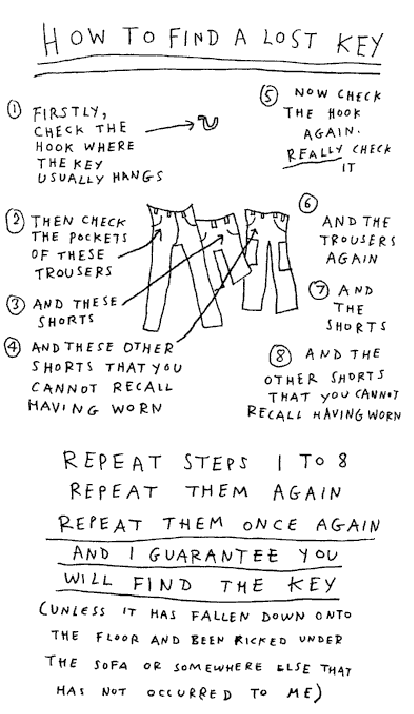
\includegraphics[scale=0.65]{lost-keys.png}

\subsection{How to get forms signed by
College}\label{how-to-get-forms-signed-by-college}

From time to time, you will need to get a form signed by your College.
Here's how:

If you need a form signed by the ``Tutor for Graduates'' (who in Exeter
College is also known as the Academic Dean -- see below), then hand it
to the Porters' Lodge or the College Office, FAO the Academic Dean, with
a short cover note explaining what you want done, and to whom the form
should be sent next (i.e.~returned to you, sent to someone else for
signing, etc.). These forms will include things like: Transfer of
Status, Confirmation of Status, Appointment of Examiners. Forms are
usually signed and returned quite quickly; but it's best not to leave
things to the last minute to get signatures!

If you need a form signed by someone else on behalf of College, then
drop it in at the Porters' Lodge for them, or contact them in advance if
you have a query. If you are not sure who needs to sign something,
please drop it into the College Office to seek help.

\subsection{Medical Information}\label{medical-information}

\paragraph{The way it works}\label{the-way-it-works}

Health services for students are basically free, as students are covered
by the NHS (the National Health Service). This means that you can go
make an appointment with a doctor, be admitted to hospital, or go to
A\&E (Accidents and Emergencies, also known, rather worryingly, as
``Casualty'' = the Emergency Room) at the hospital free of charge.

The first port of call outside of an emergency is the GP, General
Practitioner, who can deal with most ailments and can write
prescriptions. All prescriptions cost �7.65 per course of treatment,
regardless of the actual amount of medicine (i.e.~it can be one box or
10 for the same price, as long as it's the same course of treatment). If
the GP cannot deal with the issue, he will refer you to a specialist.
Note, however, that some prescriptions, such as contraception, are made
\emph{completely free of charge}.

If it's an emergency, the number to dial is 999. This will get you an
ambulance (if you are in a genuine emergency situation, ambulances do
not charge for a call-out). If you need to go to A\&E but you don't
require an ambulance, the easiest way is to call a taxi (info on this is
given below in a separate section). The Oxford hospital is called the
John Radcliffe, or the JR for short, and is located in Headington:
\url{http://www.oxfordradcliffe.nhs.uk/aboutus/hospitals/jr.aspx}.

If it is not an emergency, but you need urgent medical advice (or think
you need to see a doctor urgently) out of working hours, you should ring
your GP's surgery. You will be connected to the Out of Hours Service and
a local on-duty GP will telephone you back, usually pretty rapidly. If
you need to be seen, you will probably be directed to the Out of Hours
Centre, which is located at Manzil Way (off Cowley Road).

If you have an ailment that may not be serious enough to bother a doctor
with, but for which you still want some advice, then you can consult a
pharmacist. Pharmacies can give simple medical advice and offer you some
medicines without prescription, including emergency contraception.
Pharmacies are also the places to go to collect your prescription, if
your GP prescribes some medicine for you. Some pharmacies are open out
of hours, and can give advice when a doctor is not open (for example, on
the weekend, or on a public holiday). The closest pharmacies to the main
College site are located inside Boot's (Cornmarket St) and Boswell's
(Broad St/Cornmarket St); the closest to Exeter House are Jenner's (East
Oxford Health Centre, Manzil Way), and Boot's (Cowley Road)

The NHS also run a website, called NHS Direct
(\url{http://www.nhsdirect.nhs.uk}), that allows you to check symptoms,
and get reliable information on conditions, treatments, `what to do
next', etc.

As well as public medicine, there is also a private hospital in Oxford,
but this is very expensive if you don't have private health insurance.

For more information, see the University pages on Health:
\url{http://www.ox.ac.uk/students/shw/health/}

\paragraph{Our doctors}\label{our-doctors}

As a student at Exeter, you are required to register with the College
Doctor, or another GP practice in Oxford, unless you are given explicit
permission by the College not to do so. The default option is for you to
register with the College Doctor:

\begin{verbatim}
Dr Kenyon & Partners
19 Beaumont Street Surgery
19 Beaumont Street
Oxford
OX1 2NA
TEL: 01865 240501
FAX: 01865 240503
<http://www.19beaumontstgp.nhs.uk>
\end{verbatim}

\textbf{Registration forms, on the College's Graduate Freshers' Weblearn
pages, need to be filled in and returned directly to the doctor (not the
College) before you arrive in Oxford.}

Your induction during Freshers' Week in college will include a talk from
a representative of the surgery, so you'll get a lot more information
about this.

Although 19 Beaumont Street Surgery is known as the ``College Doctor'',
it is worth remembering that their service to you is \textbf{completely
confidential}: they will not say anything about your healthcare to the
College, or your Department, or indeed anyone else, unless you
explicitly authorise them to do so. They are the College Doctor because
they guarantee NHS registration to every Exeter College student, and
they are experienced in dealing with many of the issues that Oxford
students have (they are also very experienced at writing helpful reports
if your studies have been affected by your health). As well as being the
main doctor for Exeter College, and for seven other Oxford Colleges,
they also have a lot of non-student patients, too. Spouses and dependent
family members of Exeter students are also eligible to register for the
NHS and College doctor.

It is also worth noting that regular appointments can be very hard to
come by at short notice, and the earliest you might be offered could be
several days away. \textbf{If you want a same-day appointment}, call the
Surgery at 8 am sharp (i.e.~just as the surgery opens in the morning),
as emergency appointments and cancellation are released daily at that
time.

\paragraph{Our dentist}\label{our-dentist}

If you need a Dentist, you can use Studental. However, the College makes
no requirement to register with a dentist, and many students keep their
dentist back home as their regular dentist:

\begin{verbatim}
Studental
Helena Kennedy Student Centre
Oxford Brookes University
Headington Hill Campus
Headington Road
Oxford
OX3 0BP
<reception@studental.co.uk>
TEL: 01865 484608
\end{verbatim}

When you phone for an appointment you just need to say which college you
are from and to take your student card with you as proof. There are
leaflets about Studental outside the Exeter College nurse's room
(Staircase 7, ground floor).

\paragraph{The College nurse}\label{the-college-nurse}

The College nurse, Sarah Dragonetti, deals with minor ailments,
dressings etc. She is on duty on most days of the week, and can be found
in room 7:1 or contacted on 01865 279639.

\paragraph{First aid}\label{first-aid}

Emergencies requiring First Aid should be notified as soon as possible
to the Lodge (01865 279600) or to the appropriate Hostel Warden. (Lists
of First Aiders are also published on notice boards around the college
premises, and include the lodge staff, the Junior Dean, and the
Assistant Junior Dean.)

Emergency Medical boxes are kept at College in the Lodge, the Kitchen
and the College Office, and at Exeter House and Stapeldon House.

In medical emergencies when First Aid is not adequate arrangements will
be made by the Duty Porter to transport the patient to hospital.

\paragraph{Other health issues}\label{other-health-issues}

For eye emergencies, call the Oxford Eye Hospital in the JR. The 24 hour
emergency number is 01865 234800.

The GUM (Genito-Urinary Medicine) clinic is in the Churchill Hospital,
which is part of the JR complex.

Contraception is available free from the doctors or at the Alec Turnbull
Clinic on Cowley Road. A condom machine is located at the bottom of
Staircase 6. Limited emergency supplies will be kept in the MCR
washroom.

While it's possible to go see an NHS (i.e.~free) physiotherapist, the
waiting times are generally very long for this, and most people see
private physios. There are a number of those in Oxford, and if you ask
around you can probably get to see a very good one!

\subsection{Bikes}\label{bikes}

Cycling is a very convenient way to get around town.

To get a bike, you could buy it new or second hand from the many bike
shops around town: Bike Zone in the city centre on St.~Michael Street,
Reg Taylor Cycles on Iffley Road 3 minutes' walk from Exeter House (in
the direction away from the city), a number of shops on Cowley
(Cycloanalysts and Beeline are particular favourites, students report
that they prefer these to Cycle King). It is worth shopping around for
special start-of-term deals, which usually include a helmet, a lock, and
lights. The Oxford Union also do an annual start-of year bike sale, and
there are many bikes being sold person to person on the internet
(\url{http://www.dailyinfo.co.uk} is a popular site for such things). As
bike theft is one of the most common crimes in Oxford, it is worth
investing in a strong D-lock rather than a simple chain. If your bike is
stolen, please report it to the Police on their non-emergency number
(dial: 101); if you see a theft in progress, then please call the Police
emergency number (999).

In order to leave your bike at Exeter House or Exeter College, you must
register it at the Porters' Lodge on Main Site. They will provide you
with a sticker and number to identify your bike.

Remember: you are legally obliged to use lights after dark, and the
police like to apprehend cyclists without lights. The requirements are:
a white light (not green or amber) at the front, red at the rear; both
affixed to your bicycle and not to you or your backpack; both working,
and both conforming with required standards. A helmet is not a legal
requirement, but is definitely recommended. It's against the law in the
UK to cycle on pavements (unless there are signs indicating that
bicycles are allowed), and in pedestrianized streets (like Cornmarket
and Queen Street during the daytime -- the police like to apprehend
cyclists here, too), so please leave the pavements for people on foot.
Also, if you're unused to cycling on the left and especially to
navigating UK round-abouts (especially The Plain, which is a big 5-exit
roundabout part-way between Exeter House and the main College site), be
extra careful. Don't be shy to ask other MCR members or you college
parents to walk you through things or cycle with you the first time!

The official statement of law on cycling in Great Britain (the Highway
Code) is available at
\url{https://www.gov.uk/rules-for-cyclists-59-to-82}. A useful guide to
cycling in Oxford has been produced by local organization Cyclox:
\url{http://www.cyclox.org/cycling-in-oxford/}

If you do buy a bike and it is damaged or otherwise immobilised, Back on
Trax offer an excellent pick-up and repair service with reasonable
prices. Details at \url{http://www.backontrax.co.uk}. There is also a
Bike Doctor at the University Club, on Mansfield Rd. near the science
campus, on Wednesdays from 10am-4pm. Arrive early.

\subsection{Taxis and buses}\label{taxis-and-buses}

There are two kinds of taxis available in Oxford. One kind is the
London-style cab (called ``Hackney Carriages'') that you can hail off
the street. These have an orange light on the front when they are
available for hire. The other kind, which tends to be substantially
cheaper than Hackney Carriages, is called the private hire vehicle: this
is the one that you need to call to book your journey. At night it is
often better to ring up and book a journey than to walk onto the street
and try to hail a cab; not only are you more likely to get a car, but
this is also generally a safer alternative, as your call is recorded,
and the journey is registered. There are lots of radio-cab companies in
Oxford, and you can call them at any time of day or night. Two examples
of numbers you can call are 01865 77 88 66 (Royal Cars --
\url{http://www.royal-cars.com/royalcars}) a well-recommended company),
and 01865 24 24 24 (001 Taxis). If you have worries about taxi safety,
here is how to make a complaint:
\url{http://www.oxford.gov.uk/PageRender/decB/TaxisSafetyandComplaints}.

OUSU also runs a service called the Safety Bus, a minibus service run by
volunteers. To use the service simply ring 07714 445050 between 9
p.m.--3 a.m. Monday to Saturdays and 9 p.m.--1 a.m. on Sundays. The bus
will pick you up and deliver you to any destination within the ring road
for �1 donation per trip. Priority will always be given to vulnerable
people and individuals as the emphasis for the scheme is on safety.
However, the bus is not always available: as the service depends on
volunteers, it is not able to run on nights when volunteers are not
available to help out; in addition, there is only one bus, and many
people who want to use it.

Buses in Oxford run on a radial pattern: from the outskirts into the
centre and back. The bus that goes down Iffley Road is number 3 to Rose
Hill (N3 at night), and the closest stop to Exeter House is called
Magdalen Road. A single trip to the centre is �1.80, but it's possible
to buy season tickets and other package deals. The bus runs every 7-8
minutes during the day and every 15 minutes at night, On weekdays, the
last day bus back down Iffley Road towards Rose Hill leaves the Bonn
Square stop number D4 at 23.50 -- one additional, more expensive
nightbus (N3) leaves at 00.10. On Friday and Saturday nights, the N3
will contintue to depart from Bonn Square half hourly until 03.10. As
routes and timetables do change from time to time, please check
\url{http://www.oxfordbus.co.uk} and \url{http://www.stagecoach.com} for
the most up to date information.

\subsection{Mobile phones}\label{mobile-phones}

You effectively have three options:

\begin{enumerate}
\def\labelenumi{\arabic{enumi}.}
\itemsep1pt\parskip0pt\parsep0pt
\item
  Pay-as-you-go, which costs more per minute but requires no bank
  account to set up. Buy a SIM card and handset and you're good to go!
\item
  Pay monthly. You can typically cancel these with one month's notice,
  and they offer better rates than pay-as-you-go. Great if you leave the
  country for the summer, or are only here for a year. You will need a
  bank account and credit check.
\item
  Contract (typically 18 or 24 months). These offer best deals, and are
  the cheapest way to get a smart phone, but require some commitment, a
  bank account and credit check.
\end{enumerate}

Shop around for the best deal, and be patient. If you need a phone now
and don't have a bank account, you can pick up cheap pay-as-you-go
handsets for the short term.

The highest concentration of phone shops is on and around Cornmarket
Street, where there is a Carphone Warehouse, a Three shop, Phones4U
(though this has very mixed reviews), a Vodaphone shop, and an Orange
shop. There is also an Orange shop in the Westgate Centre, an Apple
store in Westgate and an O2 store in the Clarendon Centre.

Signal in Oxford is passable, and Vodafone along with O2 have the best
reputation for good coverage here. Inside many buildings, however, which
unfortunately includes Exeter House, you will have intermittent or no
reception. Many rooms have reliable `hot spots' in window sills and the
likes. Find yours!

\subsection{Shopping}\label{shopping}

The main grocery stores in Oxford are Tesco and Sainsbury's. Opening
times for most city grocery shops are from about 7 in the morning till
11 or 12 at night. Sunday opening hours are substantially reduced, often
open between 11 in the morning until about 5 in the afternoon.
Nevertheless, there are a few small shops (Sainsbury's in particular)
that have the same opening schedule on Sunday as on weekdays, i.e.~until
11 pm (on the Plain) or midnight (on Magdalen Street). For fresh
produce, also check out the friendly grocers in the Covered Market, the
local farmers' markets on Saturday mornings behind the Tesco on Cowley,
and the market every 1st and 3rd Thursday of the month on Gloucester
Green. For good prices on fruit and veg, go to the Gloucester Green
Wednesday market.

The main health and hygiene shop is Boot's, and there are big branches
on Cornmarket and on Cowley. Boot's and Boswell's, on Cornmarket also
include pharmacies.

For random household stuff, go to Boswell's on Broad Street, or Argos on
New Inn Hall Street off of Bonn Square. It's also worth taking a look at
Poundland in the Westgate Centre for an inexpensive if erratic spread of
household items, toiletries, humorous gifts, and snacks.

The main academic bookshop is Blackwell's on Broad Street.

Oxford also has a good selection of charity shops, which offer
inexpensive second-hand clothing and books in aid of various charities.
Oxfam has well-stocked second-hand bookshops on St Giles' (near the
Eagle \& Child pub) and in Turl Street. Cowley Road (near Exeter House)
and Headington both have several useful charity shops.

\subsection{Welfare}\label{welfare}

Welfare is Oxford's term for the various support structures in place
that serve to deal with students' problems, whatever these may be. This
section will focus mainly on the College's welfare system, but will also
mention some University-wide schemes.

\paragraph{MCR Graduate Welfare
Officer}\label{mcr-graduate-welfare-officer}

The MCR Graduate Welfare Officers are Esther Kwan and Ben Cousins. They
represent and deal with the general concerns of all members of the
graduate community in the areas of welfare, personal security,
accommodation and academic needs. They can be contacted by email at
\url{mailto:welfare@exetermcr.org}.

\paragraph{Tutor for Graduates}\label{tutor-for-graduates}

The Academic Dean (Dr Chris Ballinger) is the College's Tutor for
Graduates. He is responsible for the academic and personal welfare of
graduate students in the college, and he can be contacted at
\url{mailto:academic.dean@exeter.ox.ac.uk} and 79678 on the internal
telephone (add `01865 2' if you are calling from outside of the
university phone network, for example from a mobile phone). His College
room is high above the Porters' Lodge on Staircase 1. Dr Ballinger is
happy to see any graduate student who wishes to consult him.

You will also be assigned a College Adviser, who will be a Fellow
(senior academic professor) of the College who is working in a similar
academic area to you, and to whom you can direct any academic or other
issues.

\paragraph{Women's Adviser}\label{womens-adviser}

The Women's Adviser (Ms.~Jeri Johnson, Staircase 4:1, internal tel.
79608) is available to assist with the personal or academic difficulties
of women students at Exeter.

\paragraph{Chaplain}\label{chaplain}

The College Chaplain (Andrew Allen,
\url{mailto:chaplain@exeter.ox.ac.uk}) offers counsel and pastoral
support to all members of Exeter College, regardless of their religious
beliefs. The Freshers' Fair will also include representatives from the
different spiritual communities at Oxford.

\paragraph{Tea and Cakes}\label{tea-and-cakes}

The Welfare Officer holds a Tea and Cakes event every Friday in the MCR
at 4 pm. All members of the MCR are invited. There is ample cake, tea,
coffee, cheese, fruit, etc. hopefully something to everyone's taste.
This is a good opportunity to catch up with people (or make new
friends), and chill out at the end of the week.

\paragraph{Peer Support}\label{peer-support}

The list of peer supporters is available on various notice boards around
college. You can see a list of peer supporters at
\url{http://exetermcr.org/peer-supporters}.

\paragraph{Financial aid}\label{financial-aid}

There is a lot of financial aid available from various sources, and
announcements for scholarship applications are frequently circulated on
the mailing lists. The University prospective student pages have a
number of resources on them, as do the college funding pages. Here, we
draw your attention to three types of college-based funding.

\subparagraph{Graduate Scholarships}\label{graduate-scholarships}

The College offers various scholarships. Special attention should be
drawn to the Amelia Jackson Scholarships, which are available to
existing Exeter graduates only. The studentship pays College fees,
University fees up to the ``Home/EU'' rate, and a maintenance grant for
a period of one year. Usually two to three awards are granted each year.
It is advertised early in Trinity Term: keep an eye out for it.

\subparagraph{Grants for travel and
conferences}\label{grants-for-travel-and-conferences}

The College makes grants to enable graduate students to travel to
conferences related to their research. Forms are available on the
College website:
\url{http://www.exeter.ox.ac.uk/currentstudents/office/forms}.

\subparagraph{Hardship grants}\label{hardship-grants}

It is a condition of admission that graduate students can demonstrate
that they are able to meet the full expenses of their intended course;
Mention that, though there is some time to do paid work, there is very
little, and no one can expect to have time to ``work their way through
College'' as a graduate student at Oxford, especially as the vacations
are for scademic work, not for paid employment. However, in special
cases the College can also make grants and loans to alleviate genuinely
unexpected financial hardship. Forms can be found in our `downloads'
section or on the internal pages of the Exeter College website. The
University also has limited hardship funding:
\url{http://www.ox.ac.uk/feesandfunding/graduates/targetedsupport/hardship/}.

\paragraph{Nightline}\label{nightline}

Nightline 01865 (2)70270 is a confidential listening, support and
information service run by students for students, operating between 8pm
and 8am every night from 0th week to 9th week. You can either call them
(or drop into their office at 16 Wellington Square); they can call you
back and you can talk about anything that might be bothering you.

\paragraph{The Student Advice Service}\label{the-student-advice-service}

The Student Advice Service is a confidential listening and advice
service and aims to provide a space for students to talk over their
worries in confidence, and to offer advice on a range of issues which
students might encounter during their time at Oxford. Members of the
service can provide you both with practical advice as well as with
support for personal issues. The advisers are all experienced in dealing
with students and are committed to helping you in a supportive
environment. The Service runs during office hours and you can either
drop into OUSU at Thomas Hull House on New Inn Hall Street (although you
might have to wait for the appropriate member of the service to be free)
or make an appointment by calling OUSU on 01865 288450/1 or by emailing
\url{mailto:advice@ousu.org}.

\paragraph{Other resources}\label{other-resources}

Other welfare resources are available on the Oxford Welfare Services
website. Another resource worth keeping in mind is the OUSU Mind Your
Head Campaign: \url{http://mindyourheadoxford.wordpress.com/}

\subsection{Graduation}\label{graduation}

It may seem odd to have a message about graduation in a guide aimed at
people who have yet to start their course. However, there is nothing
like planning ahead! And thinking about this is especially important if
you are on a 1-year course and want to arrange for family and friends to
travel to Oxford to celebrate with you when you finish your course.

Students (apart from trainee medical doctors) are not told a specific
date on which they will graduate; rather, they need to book a preferred
date (which must be after their results have been confirmed!). In the
past it was quite difficult to get a date for a degree ceremony except
long in advance; but a new system has made booking easier. Taught course
students will, in the November of the last academic year of their
course, receive an invitation to book a date for their graduation. They
will then be able to book a date on which they would like to graduate,
so that they (and their families) can plan ahead. Research students
cannot plan quite so precisely when their degree will be complete, so
they will receive a booking invitation once they have ``leave to
supplicate'', which is the confirmation that they have passed their
degree course.

\section{Contact Information}\label{contact-information}

\begin{itemize}
\itemsep1pt\parskip0pt\parsep0pt
\item
  Freshers' Rep: Esther Kwan,
  \url{mailto:freshers-representative@exetermcr.org}
\item
  President: Challenger Mishra, \url{mailto:president@exetermcr.org}
\item
  VP: John Nickerson, \url{mailto:vice-president@exetermcr.org}
\item
  Treasurer: Francisca Gale, \url{mailto:treasurers@exetermcr.org}
\item
  Welfare Officers: Esther Kwan and Ben Cousins,
  \url{mailto:welfare@exetermcr.org}
\item
  Social Secretaries: Andreas Harris, Joe Tarrant and Imogen Parry,
  \url{mailto:social@exetermcr.org}
\item
  IT Officer: Abhishek Dasgupta, \url{mailto:it@exetermcr.org}
\end{itemize}

\subsection{Glossary}\label{glossary}

MCR : Middle Common Room, refers both to the actual room, and to the
graduate student body.

JCR : Junior Common Room, refers both to the actual room, and to the
undergraduate student body.

SCR : Senior Common Room, refers both to the actual room, and to the
body of College Fellows and other College officials. It is also
off-limits to students, except on special occasions like the annual
Graduate High Table in Trinity.

Battels : The termly bill that students pay to College. Main item is
rent (if you live in college accommodation), but other items could be
the catering charge, printing charges, library overdue fines, sports
levies, etc.

\textbf{We hope you have an amazing time in Oxford!}
 
\newpage
\newgeometry{left=0cm,bottom=1.5cm,right=0cm}
\thispagestyle{empty}
\large
\begin{center}
{\it Floreat Exon!}\\
\normalsize
(Let Exeter flourish)
\vfill
An electronic copy of this booklet can be found at\\ \url{http://exetermcr.org/freshers-guide}

The source for building this booklet is at\\ \url{https://github.com/exetermcr/freshers-guide}
\end{center}
\end{document}
